
%(BEGIN_QUESTION)
% Copyright 2014, Tony R. Kuphaldt, released under the Creative Commons Attribution License (v 1.0)
% This means you may do almost anything with this work of mine, so long as you give me proper credit

Anta at en differansetrykktransmitter brukes til nivåmåling i en trykksatt tank. Begge remote seals og kapillarrør er fylt med DC200 fyllvæske (spesifikk vekt = 0.934). Prosessvæsken er et hydrokarbon med tetthet 58 lb/ft$^{3}$:

$$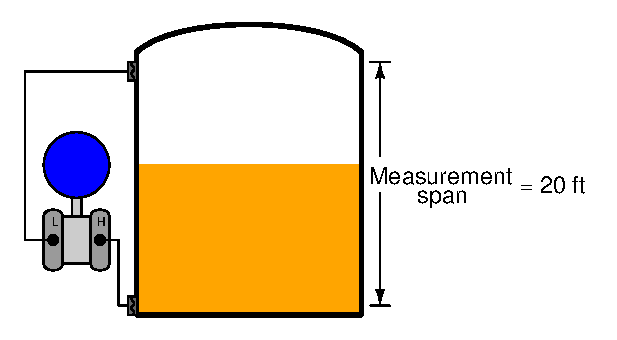
\includegraphics[width=15.5cm]{i00960x01.eps}$$

Vedlikehold vil flytte transmitteren høyere for enklere tilgang. Nå står den 6 fot over nedre remote seal, foreslått plassering er 15 fot over nedre seal. Krever dette {\it omranging} av transmitteren? Forklar. Hvis omranging kreves, er det {\it nullpunktforskyvning}, {\it spanforskyvning} eller {\it begge}?

\vskip 50pt

\underbar{file i00960}
%(END_QUESTION)





%(BEGIN_ANSWER)

5 poeng for ja/nei-svar, 5 poeng for forklaring.

\vskip 10pt

Ingen omranging trengs, fordi høydeflyttingen endrer hydrostatisk trykk likt på begge porter. Endringen er altså en {\it common-mode}-endring, ikke en differanseendring.

%(END_ANSWER)





%(BEGIN_NOTES)

{\bf Denne oppgaven er ment kun for eksamen, ikke for arbeidsark!}.

%(END_NOTES)

